%---------------------------------------------------------------------------------------------------
% Modellierung
%---------------------------------------------------------------------------------------------------
\section{Modellierung}

Das Experiment besteht grob aus drei Phasen:
\begin{itemize}
  \item Aufstieg im Ballon
  \item Absprung und freier Fall
  \item Gebremster Fall am Fallschirm und Landung
\end{itemize}
Der Aufstieg wird im Rahmen dieser Arbeit nicht weiter betrachtet.
Interessanter ist der Fall - vor allem der ungebremste Abschnitt von Absprung bis zum Öffnen des Fallschirms.
Um dies zu simulieren, müssen relevante Kräfte und Größen berücksichtigt werden. %identifiziert und modelliert werden.

Seitenwinde und mögliche Rotation werden ignoriert.
Als Masse für Springer und Ausrüstung werden $140kg$ angeommen.
Auf den Springer und seine Ausrüstung wirken lediglich zwei Kräfte:
\begin{description}
  \item[$F_g$] Zur Erde hin wirkt die Gravitation.
  \item[$F_L$] Bremsend wirkt der Luftwiderstand, der sich bei Öffnen des Fallschirms massiv erhöht.
\end{description}

Die ausschlaggebenden Größen werden im Folgenden beschrieben.

\subsection{Gravitation}
Die Gravitation wirkt zwischen dem Springer und der Erde.
Allgemein wird hier das newtonsches Gravitationsgesetz angewendet.
\begin{equation}
F_g=G \frac{m_1 m_2}{r^2}
\end{equation}
Dabei ist $G$ die Gravitationskonstante $66,7384\times 10^{-12} \frac{m^3}{kg\ s^2}$, $m_1$ und $m_2$ die beteiligten Massen und $r$ deren Abstand.
Bis auf $r$ (der Springer bewegt sich ja auf die Erde zu) sind hier alle Größen konstant.
$r$ ist dabei gleich dem Radius der Erde plus der Höhe des Springers \vgl Abb.~\ref{fig:gravitation}.
\begin{figure}[h]
  \centering
  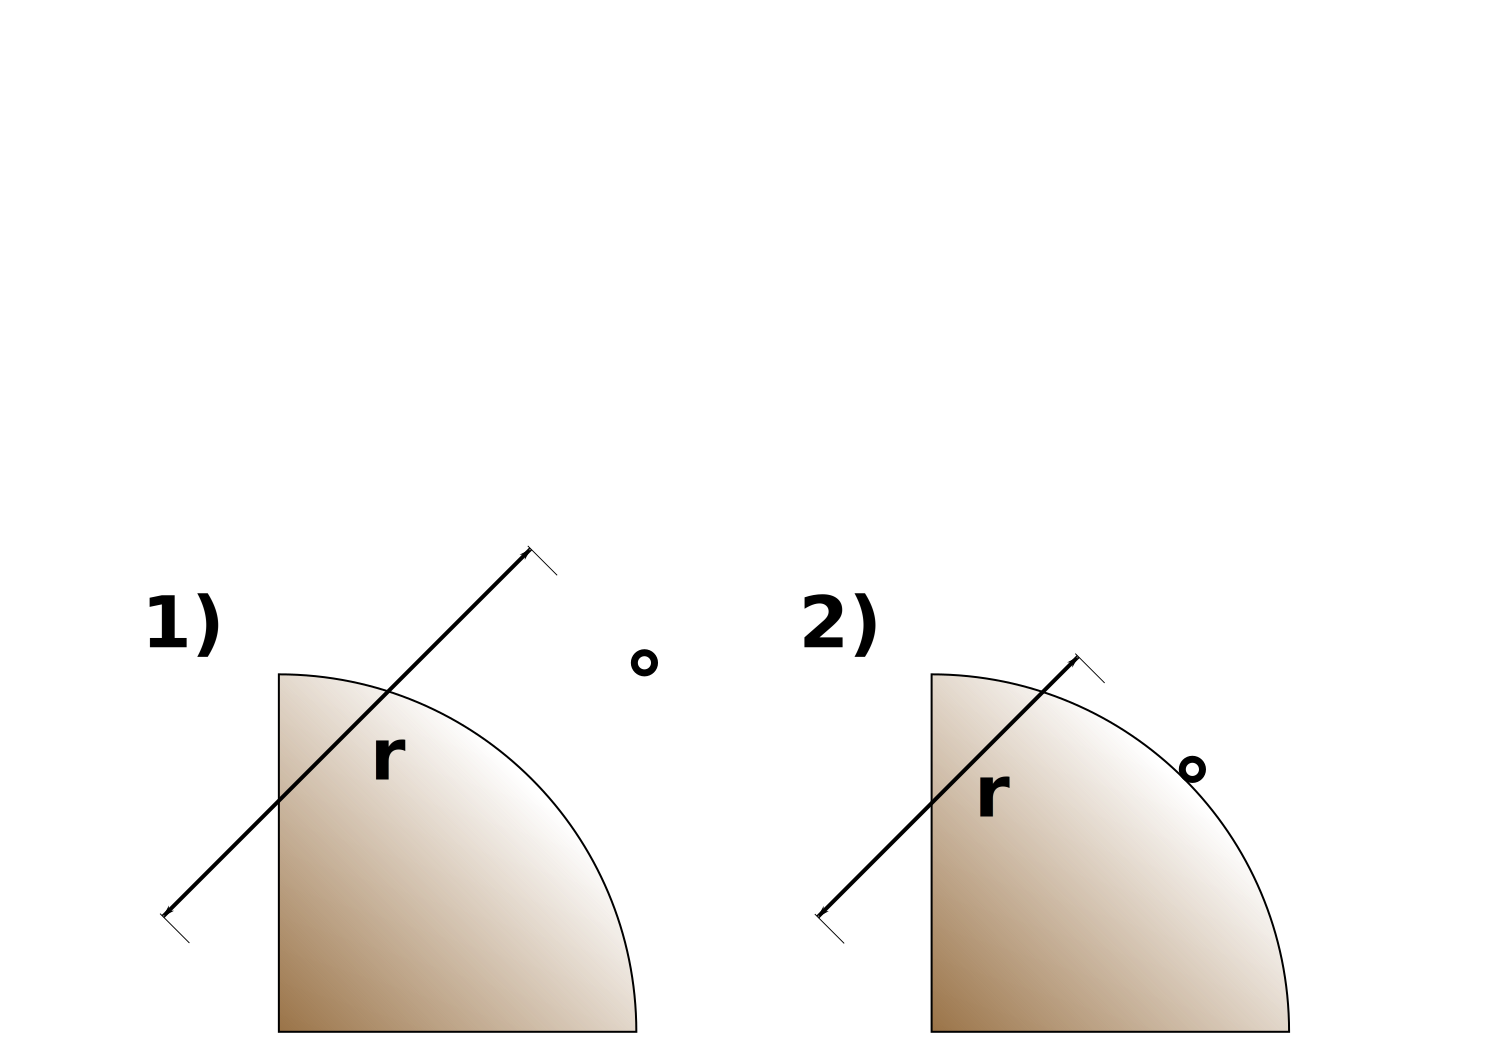
\includegraphics[width=0.5\textwidth]{gravitation}
  \caption{$r$ bei 1) Absprung und 2) Landung}
  \label{fig:gravitation}
\end{figure}

Als Erdradius wird der Äquatorradius $R_A=6.378.137m$ angenommen, als Masse des Springers $m_1=140kg$, als Masse der Erde $m_2=5,9736\times 10^{24}kg$.
Die Kraft, die auf den Springer auf Erdniveau herrscht beträgt
\begin{eqnarray}
F_{g0} &=& 66,7384\cdot 10^{-12} \frac{140\cdot 5,9736\cdot 10^{24}}{6.378.137^2} \\
 &=& 1.372 N \nonumber
\end{eqnarray}
Die Challenger zerbrach in $15km$ Höhe, der Sprung Baumgartners erfolgte aus knapp $40km$.
Um den Effekt der Höhenänderung deutlich zu zeigen wird als zweiter Wert die Gravitationskraft in $40km$ Höhe berechnet.
\begin{eqnarray}
F_{g1} &=& 66,7384\cdot 10^{-12} \frac{140\cdot 5,9736\cdot 10^{24}}{\left(6.378.137 + 40.000\right)^2} \\
 &=& 1.354,9 N \nonumber
\end{eqnarray}
Die Gravitationkraft nimmt in Absprunghöhe gegenüber der auf Erdniveau herrschenden um knapp $2\%$ ab.

\subsection{Luftwiderstand}
Der Fall des Springers wird durch den von der Atmosphäre verursachten Strömungswiderstand gebremst.
\begin{equation}
F_L=\frac{1}{2}pv^2c_wA
\end{equation}
In die Berechnung der Kraft gehen die Geschwindigkeit $v$, die Widerstandsfläche (das Produkt aus $c_w$ und $A$) und die Dichte $p$ ein.
Die Dichte der Atmosphäre ist höhenabhängig.
Die Widerstandsfläche ändert sich bei Öffnung des Fallschirms.
Weiterhin steigt die Widerstandsfläche in der Nähe der dichte- und temperaturabhängigen Schallgeschwindigkeit an.

\paragraph{Dichte und Temperatur}
Mit steigender Höhe nimmt die Dichte ab, da die darüberliegendes Gassäule kürzer wird.
Auch die Temperatur ist höhenabhängig.
Zunächste ist die Temperatur der Erdoberfläche der ausschlaggebende Faktor.
Mit zunehmender Höhe nimmt dieser Einfluss ab und die Temperatur sinkt.
Darüber nimmt die Temperatur wieder zu, da ein immer geringerer Anteil der Einstrahlung von darüberliegenden Atmosphärenschichten gefiltert wird.

Für die Simulation von Dichte und Temperatur wird das empirische NRLMSISE-00-Modell~\cite{nrlmsise00:goddardspaceflightcenter} verwendet.
Es liefert für die Parameter Datum, Uhrzeit, geographische Position und eine Höhe von 0 bis 100km Werte für Dichte und Temperatur.


\paragraph{Schallgeschwindigkeit}

